\documentclass[conference]{IEEEtran}
\usepackage[T1]{fontenc}
\usepackage{graphicx}
\usepackage{booktabs}
\usepackage{amsmath}
\usepackage{xcolor}
\usepackage{tikz}
\usetikzlibrary{positioning,arrows.meta,fit,calc,backgrounds}
\usepackage[hidelinks]{hyperref}
\usepackage{cite}

\newcommand{\cyc}[1]{#1~cycles}

\begin{document}

\title{Where Should the Work Go? Hardware/Software Partitioning and DMA Design for TinyML Inference on a RISC-V SystemC Platform}

\author{\IEEEauthorblockN{Abdelrahman Youssef}
\IEEEauthorblockA{Computer Engineering Department\\
King Fahd University of Petroleum and Minerals (KFUPM), Saudi Arabia\\
COE 407/661 System on Chip --- term paper}}

\maketitle

\begin{abstract}
This paper evaluates, at system level, how the inference time of the three MLPerf Tiny models changes as work moves from a RISC-V CPU to a DNN accelerator, and what the data movement then costs. A memory-mapped accelerator is modeled in SystemC/TLM-2.0, with its compute timing taken from the STONNE cycle-level simulator, and integrated into the RISC-V VP++ virtual prototype together with a DMA engine, a bare-metal driver and, in a final step, an interrupt controller and an arbitrated shared bus. Five steps are measured on all 48 INT8 layers: software only; a rigid 16$\times$16 mesh running the GEMMs; a flexible MAERI fabric with the same partition; MAERI with native convolution; and four DMA/bus design choices. Offloading the GEMMs gives 32.8$\times$ for ResNet-8 but only 6.2$\times$ and 5.6$\times$ for DS-CNN and MobileNet, because im2col and the depthwise layers stay on the CPU; a better compute fabric with the same partition changes the end-to-end time by less than 0.1\%. Moving convolution into the accelerator gives 1{,}389$\times$, 627$\times$ and 449$\times$ over software, after which 76--92\% of the time is DMA traffic. Double buffering then gives up to 1.28$\times$ and only hides compute; a completion interrupt costs 1.9\% on an ideal bus but is 7.5 points faster than polling on a shared bus with cycle stealing; the DMA's bus-ownership mode decides whether the CPU or the accelerator pays for contention; and the DMA burst size is the largest single lever (35\% less accelerator time from 64 to 1024-byte bursts).
\end{abstract}

\begin{IEEEkeywords}
HW/SW partitioning, DNN accelerator, SystemC, TLM-2.0, RISC-V virtual prototype, STONNE, DMA, bus arbitration, TinyML
\end{IEEEkeywords}

%=====================================================================
\section{Introduction}
A TinyML system-on-chip places a small CPU next to a DNN accelerator. Three design decisions are coupled in such a system: which part of each layer runs in hardware and which stays in software, what kind of compute fabric to build, and how the operands reach it. The cycle count of the compute fabric alone does not settle these decisions, because the layer lowering (im2col), the data transfers, the driver and the layers the accelerator cannot run all remain on the CPU and the bus.

This work measures these costs together. It integrates the STONNE accelerator simulator~\cite{stonne_cal,stonne_iiswc} as the timing engine of a memory-mapped SystemC/TLM-2.0 accelerator inside the RISC-V VP++ virtual prototype~\cite{riscv_vp_jsa,riscv_vppp}, runs bare-metal C code for every layer of the MLPerf Tiny benchmark~\cite{mlperf_tiny}, and follows the time through five steps, from software only to an accelerator whose DMA shares an arbitrated bus with the CPU. The work answers four research questions:
\begin{itemize}
\item \textbf{RQ1 (partition):} once GEMMs are offloaded, how is the remaining time split between im2col, CPU-only layers, data transfer and compute?
\item \textbf{RQ2 (fabric):} does a flexible fabric improve end-to-end time with the same partition, and what network bandwidth does it need?
\item \textbf{RQ3 (data movement):} how much do CPU copying versus DMA, and the DMA width, change the result?
\item \textbf{RQ4 (DMA and bus design):} once computation is offloaded, how much do double buffering, a completion interrupt, and the DMA's bus-ownership mode and burst size change end-to-end time and the CPU time left for other work?
\end{itemize}
The contributions are: (i) a SystemC/TLM-2.0 accelerator model with STONNE timing that compiles unchanged against SystemC 2.3.3 and 3.0 and runs inside RISC-V VP++; (ii) an end-to-end, per-phase breakdown of all 48 MLPerf Tiny layers for three accelerator designs and two HW/SW partitions; (iii) a design-space exploration of mesh size, network bandwidth, DMA width and weight sparsity; and (iv) a DMA and bus study with tiling and double buffering, an interrupt path through a PLIC, and a shared-bus contention model with burst, cycle-stealing and transparent DMA. All code, scripts and results are open source and the runs are deterministic.

%=====================================================================
\section{Background and Related Work}
This section groups the related work by the question each group answers, and states for each how this work uses or follows it.

\subsection{Modeling and exploring DNN accelerators}
Accelerator design is usually explored with models of the compute fabric and its local memories. Timeloop~\cite{timeloop} searches the mappings of a layer onto a described architecture and estimates performance and energy; MAESTRO~\cite{maestro} describes dataflows with data-centric directives and derives reuse, performance and hardware cost analytically; ZigZag~\cite{zigzag} extends the joint architecture--mapping search with uneven mappings. SCALE-Sim~\cite{scalesim} simulates systolic arrays cycle by cycle and studies how they scale. ONNXim~\cite{onnxim} simulates multi-core NPUs at cycle level with a focus on simulation speed. STONNE~\cite{stonne_cal,stonne_iiswc}, the anchor of this work, builds accelerators from a distribution network, a multiplier network and a reduction network, simulates rigid and flexible designs cycle by cycle on full DNN models and checks every result against a CPU implementation. This work uses STONNE as the compute-timing model of the accelerator and takes the parameters it exposes (fabric type, number of multipliers, network bandwidth) as design-space axes.

\subsection{Rigid and flexible compute fabrics}
The TPU~\cite{tpu} uses a large systolic array that is efficient on regular matrix multiplications. Eyeriss~\cite{eyeriss} organizes its processing elements around a row-stationary dataflow chosen to reduce data movement, which costs more energy than the arithmetic. MAERI~\cite{maeri} uses reconfigurable distribution and reduction trees so that irregular layer shapes still keep the multipliers busy, and SIGMA~\cite{sigma} adds support for sparse and irregular GEMMs through flexible interconnects and bitmap-compressed operands. This work compares a TPU-like mesh, MAERI and SIGMA, all with 256 multipliers, first alone (S0) and then inside the SoC (S2--S4).

\subsection{Evaluating accelerators in a full system}
A second group of work evaluates accelerators together with the processor, memory system and software that use them. gem5-Aladdin~\cite{gem5aladdin} couples a pre-RTL accelerator model with the gem5 system simulator to co-design accelerators and their SoC interfaces, comparing DMA and cache-coherent data movement. SMAUG~\cite{smaug} simulates deep-learning workloads end to end, from the software framework down to the accelerators and the memory system. Gemmini~\cite{gemmini} generates systolic-array accelerators and integrates them into full RISC-V SoCs built with Chipyard~\cite{chipyard}, so that operating-system and memory-system effects are part of the evaluation. SECDA~\cite{secda} co-designs FPGA accelerators for edge inference by combining SystemC simulation with execution on the FPGA, and ESP4ML~\cite{esp4ml} integrates ML accelerators into a platform-based SoC through DMA-capable accelerator sockets. This work follows the same system-level view at microcontroller scale: a STONNE-timed accelerator, a RISC-V instruction-set simulator, a bus, a DMA engine and a bare-metal driver in one SystemC simulation.

\subsection{Microcontroller-class inference}
MCUNet~\cite{mcunet} co-designs compact networks and an inference engine for microcontrollers with very small memories. GAP-8~\cite{gap8} is a RISC-V SoC for edge AI with a multi-core compute cluster, a convolution engine and autonomous DMA. XpulpNN~\cite{xpulpnn} adds RISC-V instructions for quantized networks. DORY~\cite{dory} tiles DNN layers automatically for low-cost MCUs and generates code that moves the tiles between memory levels with double-buffered DMA transfers, overlapping transfers with computation. This work runs the INT8 layers of MLPerf Tiny~\cite{mlperf_tiny} and applies the same tiling and double-buffering principle inside the accelerator (S5).

\subsection{Virtual prototypes and transaction-level modeling}
Transaction-level modeling~\cite{tlm_overview} raises the abstraction of on-chip communication from signals to transactions, which makes full-system simulation fast enough for software development and design-space exploration; SystemC and its TLM-2.0 library are standardized in IEEE 1666~\cite{ieee1666}. The RISC-V VP~\cite{riscv_vp_jsa} is an open-source SystemC/TLM-2.0 virtual prototype with an instruction-set simulator; it has been extended with the vector extension~\cite{riscv_vvp_date} and continued as RISC-V VP++~\cite{riscv_vppp}. This work adds a platform to VP++ with the accelerator, a PLIC and an optional shared-bus model, all in standard SystemC, so the same accelerator source also compiles against SystemC~2.3.3.

\subsection{DMA, interrupts and shared on-chip buses}
How a device signals completion and how it shares the bus are classic SoC design choices. Interrupts free the processor while it waits, while polling avoids the interrupt overhead; at high event rates interrupt handling itself can saturate a processor, which led to hybrid schemes that switch between the two~\cite{livelock}. On RISC-V, external interrupts reach a hart through a platform-level interrupt controller (PLIC)~\cite{riscv_priv,fe310}. On a shared bus, an arbiter decides which master is served; LOTTERYBUS~\cite{lotterybus} is one example of an arbitration scheme designed to control how bandwidth is divided between masters. A DMA engine can own the bus in burst (block) mode, transfer single words between processor accesses (cycle stealing), or use only idle bus cycles (transparent mode). This work models these three ownership modes, a completion interrupt through a PLIC, and polling, on the same platform, and measures their effect on the accelerator's time and on the CPU time left for other work (S5).

%=====================================================================
\section{Platform and Method}
\subsection{The simulated SoC}
Fig.~\ref{fig:platform} shows the platform \texttt{accel32-vp}. It is the VP++ \texttt{tiny32} platform (one RV32IM core, 32~MB memory, CLINT, syscall device) with two additions: the accelerator as a bus target at 0x1000\_0000 and its DMA as a third bus master, plus, for S5, an FE310-style PLIC~\cite{fe310} and an optional shared-bus arbiter. The CPU uses VP++'s default timing at 100~MHz: every instruction fetch, load and store goes through the bus to a 1-cycle memory, and the TLM quantum is one cycle. All times are read from a platform timer register that returns SystemC simulated time, so they include bus and memory delays.

\begin{figure}[t]\centering
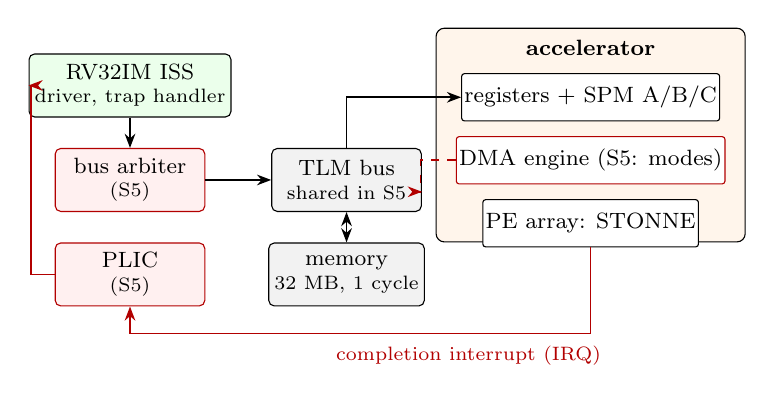
\begin{tikzpicture}[font=\footnotesize,
  blk/.style={draw, rounded corners=2pt, align=center, minimum height=8mm, minimum width=19mm, inner sep=2pt},
  new/.style={blk, draw=red!70!black, fill=red!6},
  sub/.style={draw, rounded corners=1pt, fill=white, align=center, minimum width=24mm, minimum height=6mm, inner sep=1pt},
  arr/.style={-{Stealth[length=1.8mm]}, semithick}]
\node[blk, fill=green!8] (cpu) at (0,2.4) {RV32IM ISS\\[-1pt]\scriptsize driver, trap handler};
\node[new] (arb) at (0,1.2) {bus arbiter\\[-1pt]\scriptsize (S5)};
\node[new] (plic) at (0,0) {PLIC\\[-1pt]\scriptsize (S5)};
\node[blk, fill=gray!10] (bus) at (2.75,1.2) {TLM bus\\[-1pt]\scriptsize shared in S5};
\node[blk, fill=gray!10] (mem) at (2.75,0) {memory\\[-1pt]\scriptsize 32 MB, 1 cycle};
\node[sub] (regs) at (5.85,2.25) {registers + SPM A/B/C};
\node[sub, draw=red!70!black] (dma) at (5.85,1.45) {DMA engine (S5: modes)};
\node[sub] (pe) at (5.85,0.65) {PE array: STONNE};
\begin{scope}[on background layer]
\node[draw, rounded corners=3pt, fill=orange!8, fit=(regs)(dma)(pe), inner xsep=2.5mm, inner ysep=2.5mm,
      yshift=3.2mm, label={[anchor=north, font=\footnotesize\bfseries, yshift=-0.3mm]north:accelerator}] (acc) {};
\end{scope}
\draw[arr] (cpu) -- (arb);
\draw[arr] (arb) -- (bus);
\draw[arr, {Stealth[length=1.8mm]}-{Stealth[length=1.8mm]}] (bus) -- (mem);
\draw[arr] (bus.north) |- (regs.west);
\draw[arr, red!70!black, dashed] (dma.west) -- ++(-0.45,0) |- ([yshift=-1.5mm]bus.east);
\draw[arr, red!70!black] (pe.south) -- (5.85,-0.75) -- (0,-0.75) -- (plic.south);
\draw[arr, red!70!black] (plic.west) -- ++(-0.3,0) |- (cpu.west);
\node[font=\scriptsize, red!70!black, anchor=north] at (4.3,-0.78) {completion interrupt (IRQ)};
\end{tikzpicture}
\caption{The simulated SoC. RISC-V VP++ provides the CPU, bus and memory; the accelerator is the SystemC module of this work, with compute cycles from STONNE. Red: the S5 additions.}
\label{fig:platform}
\end{figure}

\subsection{The accelerator model}
The accelerator is an \texttt{sc\_module} with a TLM-2.0 target socket (registers and three scratchpads: A and B, int8, 256~KB and 128~KB; C, int32, 256~KB) and an initiator socket for its DMA. A control thread waits for \texttt{CTRL.START}, checks that the job fits the scratchpads, loads the inputs in DMA mode, runs the job on STONNE, waits for STONNE's cycle count, stores the output in DMA mode and sets \texttt{DONE}. Two job types exist: \texttt{OP\_GEMM}, $C=AB^\top$ on any architecture, and \texttt{OP\_CONV}, a standard or depthwise convolution on MAERI with the zero padding inserted by the accelerator. The data really moves through the bus; the DMA time for a transfer split into bursts $b_i$ is
\begin{equation}
t_{\mathrm{DMA}} = \sum_i \left( L + \lceil b_i / w \rceil \right),
\label{eq:dma}
\end{equation}
with burst latency $L=10$ cycles, width $w=4$ bytes/cycle and 64-byte bursts by default. STONNE is configured as a TPU-like 16$\times$16 output-stationary mesh, as MAERI (linear multiplier network, ART reduction tree, tiles from STONNE's mapper) or as SIGMA (bitmap-compressed operands, weights stationary), always with 256 multipliers. STONNE's mapper runs a depthwise layer one channel at a time; the backend instead gives each channel $R{\cdot}S$ multipliers and runs as many channels and output columns side by side as fit, which made MobileNet's first depthwise layer about 12$\times$ faster. The model uses only standard SystemC and TLM-2.0, so the same source compiles into a unit-test bench on SystemC 2.3.3 and into VP++ on SystemC 3.0.

\subsection{Workload, partitions and verification}
Table~\ref{tab:workload} lists the workload: every CONV, pointwise (PW), depthwise (DW) and FC layer of the three MLPerf Tiny INT8 models, with fixed pseudo-random data. Two HW/SW partitions are compared. In the \emph{gemm} partition the CPU lowers convolutions with im2col and the accelerator runs GEMMs; depthwise layers stay on the CPU. In the \emph{conv} partition (MAERI only) the accelerator runs CONV and DW layers natively, and PW and FC layers as GEMMs. In every checked run, each accelerated output is compared with the CPU result, and all of them pass; the sweeps reuse checked configurations with faster program variants that skip the CPU reference and reproduce the checked runs' cycle counts. The accelerator is also tested alone, in a SystemC 2.3.3 bench, for GEMM and CONV jobs, refused job types and oversized jobs.

\begin{table}[t]\centering\footnotesize
\caption{Workload: the INT8 layers of the three MLPerf Tiny models.}\label{tab:workload}
\begin{tabular}{@{}lrrrrrr@{}}\toprule
model & layers & CONV & PW & DW & FC & MMACs\\\midrule
ResNet-8 & 10 & 9 & 0 & 0 & 1 & 12.50 \\
DS-CNN & 10 & 1 & 4 & 4 & 1 & 2.66 \\
MobileNetV1-0.25 & 28 & 1 & 13 & 13 & 1 & 7.49 \\
\bottomrule\end{tabular}\end{table}


%=====================================================================
\section{From Software to a Better Accelerator (S0--S3)}
\subsection{S0: the compute fabrics alone}
Table~\ref{tab:stonne} repeats the kind of comparison made in the STONNE paper on eight MLPerf Tiny layer shapes. The rigid mesh is well used on large regular GEMMs (94\% on ResNet-8 conv7) but drops to 19\% on MobileNet pw2, whose $K=8$ does not fill the array; MAERI with a 256-wide distribution network stays between 84\% and 100\% except on that same layer (50\%). SIGMA's cycles fall with 50\% zero weights (ResNet-8 conv1: 16{,}591 to 6{,}225 cycles) while the other two do not change.

\begin{table}[t]\centering\scriptsize\setlength{\tabcolsep}{2pt}
\caption{S0: STONNE alone, 256 multipliers each. Compute cycles and multiplier utilization (\%).}\label{tab:stonne}
\begin{tabular}{@{}llrrrrrr@{}}\toprule
layer & $M{\times}K{\times}N$ & TPU & MAERI & SIGMA & SIGMA & \multicolumn{2}{c}{util.\ (\%)}\\
 & & 16$\times$16 & bw 256 & dense & 50\% z. & TPU & MAERI\\\midrule
resnet8\_conv0 & 1024$\times$27$\times$16 & 3{,}968 & 2{,}061 & 4{,}118 & 2{,}058 & 44 & 84 \\
resnet8\_conv1 & 1024$\times$144$\times$16 & 11{,}456 & 9{,}236 & 16{,}591 & 6{,}225 & 80 & 100 \\
resnet8\_conv7 & 64$\times$576$\times$64 & 9{,}776 & 9{,}371 & 14{,}593 & 9{,}493 & 94 & 98 \\
dscnn\_conv0 & 125$\times$40$\times$64 & 2{,}388 & 1{,}271 & 1{,}520 & 946 & 52 & 98 \\
dscnn\_pw2 & 125$\times$64$\times$64 & 3{,}156 & 2{,}027 & 2{,}723 & 1{,}611 & 63 & 99 \\
mbnet\_pw2 & 2304$\times$8$\times$16 & 6{,}192 & 2{,}315 & 4{,}618 & 4{,}618 & 19 & 50 \\
mbnet\_pw14 & 36$\times$128$\times$128 & 3{,}816 & 2{,}379 & 3{,}246 & 1{,}855 & 60 & 97 \\
mbnet\_pw26 & 9$\times$256$\times$256 & 4{,}544 & 2{,}582 & 6{,}197 & 3{,}590 & 51 & 89 \\
\bottomrule\end{tabular}\end{table}


\subsection{S1--S3: end-to-end time}
Table~\ref{tab:e2e} and Fig.~\ref{fig:e2e} give the end-to-end results, and Fig.~\ref{fig:breakdown} shows where the time goes.

\textbf{S1, software.} Plain C on the ISS needs 383.3, 106.5 and 276.8~M cycles for ResNet-8, DS-CNN and MobileNet (3.8, 1.1 and 2.8~s at 100~MHz).

\textbf{S2, a rigid mesh with the gemm partition.} ResNet-8 becomes 32.8$\times$ faster with DMA, but im2col on the CPU is now 96.3\% of its time. DS-CNN and MobileNet gain only 6.2$\times$ and 5.6$\times$ because their depthwise layers, left on the CPU, take 97.0\% and 93.7\% of the time. Copying the operands with the CPU instead of the DMA costs 1.05--1.32$\times$ more.

\textbf{S3a, a flexible fabric with the same partition.} MAERI computes ResNet-8's GEMMs in 18\% fewer cycles than the mesh (49{,}590 vs.\ 60{,}669), and the end-to-end time changes by 0.1\%. This is Amdahl's law: with the CPU parts at 96--99\% of the time, the fabric cannot matter (RQ2 with an unchanged partition).

\textbf{S3b, native convolution.} Moving im2col and the depthwise layers into the accelerator gives 1{,}389$\times$, 627$\times$ and 449$\times$ over software (2.76, 1.70 and 6.16~ms per inference). The DMA load time of ResNet-8 also falls 3.3$\times$, because im2col no longer expands the input. MAERI's native convolution of ResNet-8 needs slightly more compute cycles than its GEMM form (60{,}810 vs.\ 49{,}590), yet the system is 42$\times$ faster: the partition, not the fabric, sets the end-to-end time. What remains is data movement: DMA load and store are 76\%, 90\% and 92\% of the total, and the store of the 32-bit outputs alone is 51--69\% (RQ1).

\begin{figure}[t]\centering
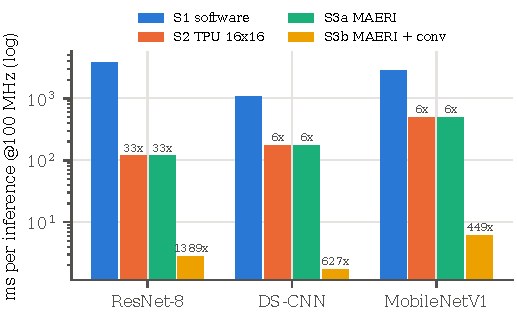
\includegraphics[width=\columnwidth]{figures/fig_e2e.pdf}
\caption{Time per inference for each step (DMA mode, log scale); labels are speedups over S1.}
\label{fig:e2e}
\end{figure}

\begin{figure}[t]\centering
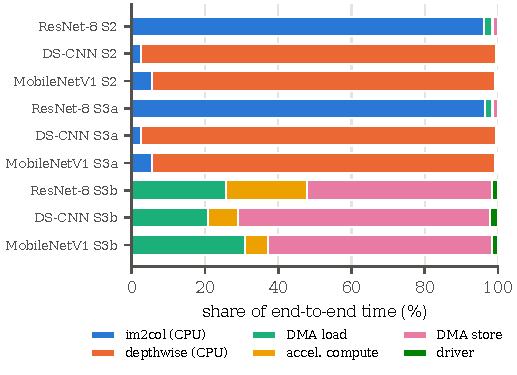
\includegraphics[width=\columnwidth]{figures/fig_breakdown.pdf}
\caption{Where the end-to-end time goes in S2, S3a and S3b (DMA mode).}
\label{fig:breakdown}
\end{figure}

\begin{table*}[t]\centering\footnotesize\setlength{\tabcolsep}{3pt}
\caption{S1--S3: end-to-end cycles (DMA mode), speedup over software, and where the time goes (\% of total).}\label{tab:e2e}
\begin{tabular}{@{}llrrrrrr@{}}\toprule
model & design & cycles & speedup & im2col & CPU-only & DMA & compute\\\midrule
ResNet-8 & S1 software & 383{,}321{,}507 & 1.0$\times$ & 0.0 & 100 & 0.0 & 0.0 \\
 & S2 TPU 16$\times$16 & 11{,}698{,}611 & 32.8$\times$ & 96.3 & 0.0 & 3.2 & 0.5 \\
 & S3a MAERI & 11{,}687{,}511 & 32.8$\times$ & 96.4 & 0.0 & 3.2 & 0.4 \\
 & S3b MAERI + conv & 275{,}915 & 1{,}389$\times$ & 0.0 & 0.0 & 76.4 & 22.0 \\
\midrule
DS-CNN & S1 software & 106{,}535{,}249 & 1.0$\times$ & 0.0 & 100 & 0.0 & 0.0 \\
 & S2 TPU 16$\times$16 & 17{,}159{,}591 & 6.2$\times$ & 2.4 & 97.0 & 0.5 & 0.1 \\
 & S3a MAERI & 17{,}153{,}911 & 6.2$\times$ & 2.4 & 97.0 & 0.5 & 0.1 \\
 & S3b MAERI + conv & 169{,}883 & 627$\times$ & 0.2 & 0.0 & 89.6 & 8.1 \\
\midrule
MobileNetV1-0.25 & S1 software & 276{,}812{,}977 & 1.0$\times$ & 0.0 & 100 & 0.0 & 0.0 \\
 & S2 TPU 16$\times$16 & 49{,}581{,}882 & 5.6$\times$ & 5.5 & 93.7 & 0.8 & 0.1 \\
 & S3a MAERI & 49{,}553{,}362 & 5.6$\times$ & 5.5 & 93.7 & 0.8 & 0.1 \\
 & S3b MAERI + conv & 615{,}968 & 449$\times$ & 0.1 & 0.0 & 91.8 & 6.4 \\
\bottomrule\end{tabular}\end{table*}


%=====================================================================
\section{Design-Space Exploration (S4)}
Fig.~\ref{fig:dse} shows four sweeps, each run on all 48 layers in DMA mode.
\begin{itemize}
\item \textbf{Mesh size} (gemm partition): from 8$\times$8 to 32$\times$32 the GEMM compute of ResNet-8 falls 9.0$\times$ (221{,}008 to 24{,}633 cycles) and the end-to-end time by 1.7\%.
\item \textbf{MAERI bandwidth} (gemm partition): from 32 to 256 elements/cycle, compute falls 6.8$\times$ and the end-to-end time by 2.4\%. In the conv partition the same bandwidth matters: 64 instead of 256 makes ResNet-8 1.31$\times$ slower (362{,}115 vs.\ 275{,}915 cycles).
\item \textbf{DMA width} (RQ3): in the conv partition 16 instead of 4 bytes/cycle makes the three models 1.54$\times$, 1.70$\times$ and 1.74$\times$ faster; in the gemm partition the same change gives 1.5\%.
\item \textbf{Weight sparsity}: SIGMA's compute for ResNet-8 falls from 89{,}228 to 43{,}090 and 14{,}665 cycles with 0, 50 and 80\% zero weights, while the TPU's stays at 60{,}669, and the end-to-end time changes by less than 0.7\%.
\end{itemize}
The common thread is that each improvement shows up end-to-end only once the part that limits the system has been removed: first the CPU work, then the data movement.

\begin{figure*}[t]\centering
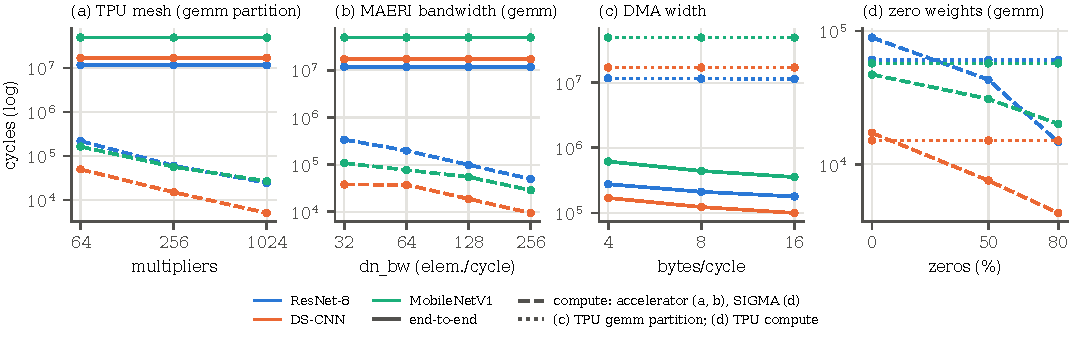
\includegraphics[width=\textwidth]{figures/fig_dse.pdf}
\caption{S4 sweeps on all MLPerf Tiny layers, DMA mode, log scale. Colour = model; line style = what is measured.}
\label{fig:dse}
\end{figure*}

%=====================================================================
\section{DMA and Bus Design (S5)}
After S3b the accelerator mostly moves data. S5 changes the data movement in three ways, all off unless the driver enables them, so S1--S4 are reproduced exactly; the one-piece DMA results of S5 equal S3b layer by layer.

\subsection{Model}
\textbf{Tiling and double buffering.} With \texttt{CTRL.TILE} a job is cut into tiles of \texttt{TILE\_ROWS} rows: rows of $A$ and $C$ for a GEMM, output rows for a convolution, whose tiles also read their halo input rows. The weights are loaded once. With \texttt{CTRL.DBUF} the control thread becomes a DMA engine and a second \texttt{SC\_THREAD} computes. The two use ping-pong halves of scratchpads A and C and synchronise through three counters (tiles loaded, computed and stored) and one event: tile $i$ is computed when it is loaded and output buffer $i \bmod 2$ is free, and the DMA loads tile $i{+}1$ and stores tile $i{-}1$ while tile $i$ is computed. With one DMA engine and one PE array, a job of $T$ tiles with weight load $W$, loads $L_i$, compute $C_i$ and stores $S_i$ obeys
\begin{multline}
\max\Big(W + \textstyle\sum_i (L_i + S_i),\ \sum_i C_i\Big) \le t_{\mathrm{DBUF}} \\
\le W + \textstyle\sum_i (L_i + C_i + S_i).
\label{eq:dbuf}
\end{multline}

\textbf{Completion interrupt.} With \texttt{CTRL.IRQ} the accelerator raises a level interrupt at \texttt{DONE}, which reaches the core's machine external interrupt through PLIC source~1~\cite{fe310,riscv_priv}. The handler claims the interrupt at the PLIC, acknowledges it at the accelerator, sets a flag and completes the claim. The waiting code masks \texttt{mstatus.MIE}, checks the flag and executes \texttt{wfi}; WFI wakes on a pending enabled interrupt even while it is masked, so no completion can be lost. The CPU then either sleeps (WFI) or runs a background task, a checksum over a buffer in memory that stands in for other application work.

\textbf{Shared bus.} An arbiter port in front of the CPU and the DMA engine reserve tenures on one bus timeline: each request gets the first free slot at or after its time that is long enough, first come first served, without pre-empting a granted tenure. The CPU holds the bus for the target's latency (memory 1 cycle). The DMA uses one of three ownership modes: \emph{block} reserves a whole transfer, \emph{cycle stealing} reserves one burst at a time, and \emph{transparent} reserves nothing, but waits until enough idle bus time has passed. Looking back at the timeline is exact, because no request can be made in the past.

\textbf{Tests.} A SystemC 2.3.3 bench checks the timing properties of~\eqref{eq:dbuf}, one interrupt per job with zero status polls, and the three ownership modes. With the CPU asleep all modes take the ideal-bus time. With a CPU that reads memory in a loop, block mode keeps the DMA at full speed and stalls the CPU for up to a whole transfer (26{,}624 cycles); cycle stealing bounds the stall to one burst (26 cycles); and transparent mode never stalls the CPU, which then completes 27$\times$ more reads, but makes the DMA job 1.93$\times$ slower.

\begin{table*}[t]\centering\footnotesize\setlength{\tabcolsep}{2.6pt}
\caption{S5a--c (checked runs). 5a: ideal bus, CPU polls. 5b: interrupt + WFI, ideal bus. 5c: shared bus, cycle stealing (64-B bursts), interrupt + background work. Time change relative to 5a; ``free'' = share of the waiting time the CPU can use.}\label{tab:step5}
\begin{tabular}{@{}llrrrrrr@{}}\toprule
 & & \multicolumn{2}{c}{5a (poll, ideal)} & \multicolumn{2}{c}{5b (WFI)} & \multicolumn{2}{c}{5c (steal + BG)}\\
\cmidrule(lr){3-4}\cmidrule(lr){5-6}\cmidrule(lr){7-8}
model & mode & cycles & vs DMA & $\Delta$\% & free\% & $\Delta$\% & free\%\\\midrule
ResNet-8 & DMA & 275{,}915 & 1.00$\times$ & +1.4 & 98 & +7.3 & 25 \\
 & TILE & 284{,}822 & 0.97$\times$ & +1.4 & 98 & +6.9 & 25 \\
 & DBUF & 229{,}542 & 1.20$\times$ & +1.7 & 98 & +8.4 & 11 \\
\midrule
DS-CNN & DMA & 169{,}883 & 1.00$\times$ & +2.3 & 97 & +9.9 & 15 \\
 & TILE & 174{,}498 & 0.97$\times$ & +2.2 & 97 & +9.1 & 15 \\
 & DBUF & 159{,}898 & 1.06$\times$ & +2.4 & 97 & +10.8 & 9 \\
\midrule
MobileNetV1-0.25 & DMA & 615{,}968 & 1.00$\times$ & +1.8 & 98 & +8.4 & 13 \\
 & TILE & 636{,}084 & 0.97$\times$ & +1.7 & 98 & +8.6 & 14 \\
 & DBUF & 594{,}404 & 1.04$\times$ & +1.8 & 98 & +9.1 & 9 \\
\bottomrule\end{tabular}\end{table*}


\subsection{Results}
Table~\ref{tab:step5} gives the checked runs and Table~\ref{tab:bus} and Fig.~\ref{fig:step5} the sweeps (RQ4).

\textbf{Double buffering hides only compute.} It makes ResNet-8 1.20$\times$ faster at 4~bytes/cycle, rising to 1.25$\times$ and 1.28$\times$ at 8 and 16, because a faster DMA leaves the compute a larger share to hide. DS-CNN and MobileNet gain 1.04--1.13$\times$, since their time is almost all the output store; by~\eqref{eq:dbuf}, overlap cannot hide the DMA itself. Tiling alone costs about 3\%: each tile pays its own STONNE pipeline fill and convolution tiles re-read their halo rows. The best tiling is coarse, four tiles for ResNet-8 (0.78 of the one-piece time at 16~bytes/cycle) and two for the other models; with 16 tiles at 4~bytes/cycle MobileNet becomes 1\% slower than without tiling.

\textbf{The interrupt pays off when the bus is shared.} On the ideal bus, polling is fastest: the interrupt adds 1.4--2.4\% because the CPU reacts after about 186 cycles (PLIC, trap entry, register saves, claim) instead of about 33, but 97--98\% of the waiting time becomes free and the 27{,}162--60{,}515 status reads per model disappear. With cycle stealing, a polling CPU takes bus slots from the DMA (97{,}376 cycles of DMA waiting), and polling becomes 9.7\% slower than on the ideal bus, while interrupt + WFI stays at +2.2\%. With transparent DMA, a polling CPU nearly starves the DMA (+63.7\%), and WFI leaves the DMA the whole bus (+2.0\%).

\textbf{Each ownership mode suits a different CPU.} Block mode keeps the accelerator at full speed whatever the CPU does (+0.1\% with polling) but freezes the cacheless CPU for up to 26{,}624 cycles at a time, even on its way to WFI, so only 21\% of the waiting time is free. Cycle stealing bounds every stall to one burst, but the busier master loses: background work gets 10\% of the CPU. Transparent mode leaves 86\% of the CPU to background work and makes the inference 80\% slower. For this SoC, interrupt + WFI stays within 2.2\% of the ideal bus with polling in every mode, and the ownership mode matters only when the CPU has other work.

\textbf{The burst size is the largest lever.} With 64-byte bursts the fixed latency in~\eqref{eq:dma} is 10 of every 26 cycles. Bursts of 1024 bytes cut the accelerator time of all three models from 0.97 to 0.63~M cycles (block mode, busy CPU), more than double buffering gains. The price is the CPU's worst-case response: in block mode the longest stall is a whole transfer (17{,}024--180{,}224 cycles); with cycle stealing it is one burst, 11 cycles at 4-byte bursts and 266 at 1024-byte bursts, so 1024-byte cycle stealing is as fast as block mode with a 64$\times$ shorter worst-case stall.

\begin{table*}[t]\centering\footnotesize\setlength{\tabcolsep}{3pt}
\caption{Bus ownership $\times$ how the CPU waits: double-buffered jobs, 64-B bursts, all three models together. $\Delta$ relative to the ideal bus with polling.}\label{tab:bus}
\begin{tabular}{@{}llrrrrr@{}}\toprule
bus & CPU waits by & cycles & $\Delta$\% & free\% & max CPU stall & DMA bus wait\\\midrule
ideal & poll & 983{,}844 & +0.0 & 0 & 0 & 0 \\
 & IRQ + WFI & 1{,}002{,}615 & +1.9 & 98 & 0 & 0 \\
 & IRQ + BG & 1{,}009{,}728 & +2.6 & 85 & 0 & 0 \\
\midrule
block & poll & 984{,}674 & +0.1 & 0 & 26{,}624 & 773 \\
 & IRQ + WFI & 1{,}004{,}239 & +2.1 & 21 & 26{,}624 & 316 \\
 & IRQ + BG & 1{,}019{,}258 & +3.6 & 3 & 26{,}624 & 947 \\
\midrule
cycle steal & poll & 1{,}079{,}494 & +9.7 & 0 & 26 & 97{,}376 \\
 & IRQ + WFI & 1{,}005{,}740 & +2.2 & 95 & 26 & 1{,}989 \\
 & IRQ + BG & 1{,}074{,}523 & +9.2 & 10 & 26 & 62{,}038 \\
\midrule
transparent & poll & 1{,}610{,}424 & +63.7 & 0 & 0 & 634{,}740 \\
 & IRQ + WFI & 1{,}003{,}911 & +2.0 & 98 & 0 & 1{,}296 \\
 & IRQ + BG & 1{,}771{,}104 & +80.0 & 86 & 0 & 768{,}126 \\
\bottomrule\end{tabular}\end{table*}


\begin{figure*}[t]\centering
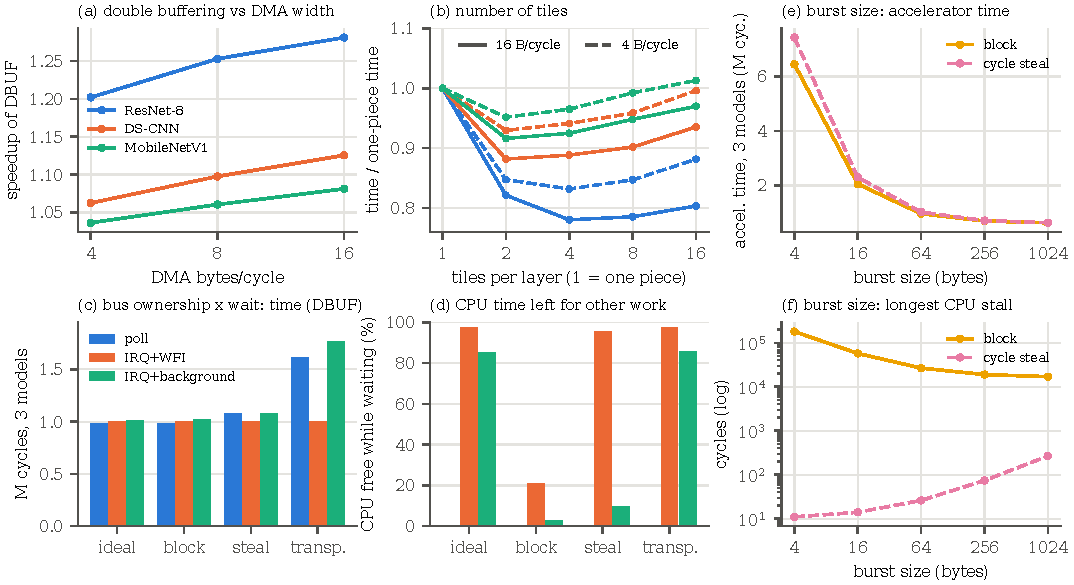
\includegraphics[width=\textwidth]{figures/fig_step5.pdf}
\caption{S5 sweeps on all layers, conv partition. (a) Speedup of double buffering over the one-piece job. (b) Time against tiles per layer. (c, d) Inference time and CPU time left free for each bus model and wait style (double-buffered jobs, 64-B bursts). (e, f) Burst size with a busy CPU: accelerator time and the longest single CPU stall.}
\label{fig:step5}
\end{figure*}

%=====================================================================
\section{Insights}
The measurements lead to seven insights. Each is stated in plain terms with the number that supports it.

\begin{enumerate}
\item \textbf{Speeding up a part that is not the bottleneck changes nothing.} In S3a the accelerator computed 18\% faster, and the inference time changed by 0.1\%, because 96--99\% of the time was CPU work (im2col and depthwise layers). The first question for any accelerator is what share of the time it can remove (Amdahl's law).
\item \textbf{Where the work runs matters more than how fast the engine is.} Moving convolution and depthwise layers into the accelerator (S3b) made ResNet-8 42$\times$ faster than S3a, although the accelerator's own compute became slightly slower (60{,}810 vs.\ 49{,}590 cycles). The HW/SW partition was the most important design decision in this study (RQ1).
\item \textbf{Each improvement moves the bottleneck.} In S2 the bottleneck is CPU work; after S3b it is data movement (76--92\% of the time); in S5 it becomes bus sharing and burst overhead. A design is limited by the part it has not addressed yet, so design-space exploration has to be repeated after every change.
\item \textbf{Once compute is cheap, data movement is the cost.} After S3b, a 4$\times$ wider DMA gave 1.54--1.74$\times$, a larger network bandwidth gave 1.31$\times$, and the largest single cost was writing back 32-bit outputs (51--69\% of the time). In the gemm partition the same DMA change gave 1.5\% (RQ2, RQ3).
\item \textbf{Overlap only hides what can run in parallel.} With one DMA engine, double buffering hides the compute behind the transfers and nothing else, as Eq.~\eqref{eq:dbuf} bounds. It gave 1.20--1.28$\times$ for ResNet-8, where compute is 22\% of the accelerator time, and 1.04--1.13$\times$ for the models whose time is almost all transfers. A few large tiles were best, because each tile adds pipeline fill and halo reads.
\item \textbf{An interrupt does not make a job faster; it frees the CPU.} On an ideal bus, polling was 1.4--2.4\% faster. The interrupt is worth its 186-cycle reaction when the CPU has other work, or when the bus is shared: a polling CPU then takes bus slots from the DMA (+9.7\% versus +2.2\% with cycle stealing; +63.7\% versus +2.0\% with transparent DMA).
\item \textbf{The DMA's bus policy decides who waits.} Block mode protects the accelerator and freezes the CPU for up to 26{,}624 cycles; transparent mode protects the CPU and slows the inference by up to 80\%; cycle stealing bounds every CPU stall to one burst. Larger bursts make the DMA faster (35\% less accelerator time from 64 to 1024 bytes) but lengthen each stall, so the burst size trades throughput against real-time response; 1024-byte cycle stealing matched block-mode speed with a 64$\times$ shorter worst-case stall (RQ4).
\end{enumerate}

\section{Limits}
The software baseline is plain C on a slow, cacheless core, so absolute speedups over S1 are large; the comparisons between designs use the same CPU, bus and data. The DMA timing is analytical and the shared bus has no split transactions, so a burst holds the bus for its latency. Without a CPU cache, every instruction fetch uses the bus, which is the worst case for contention. Transparent mode uses every idle bus cycle and is therefore optimistic. Compute cycles come from STONNE's model, so no area or power is claimed. Each layer runs on fresh random data, and pooling, residual additions and requantization are not included. Natural next steps are requantizing outputs to INT8 inside the accelerator, which shrinks the dominant store by 4$\times$; a second DMA channel so that loads and stores overlap; and a CPU cache to measure how much contention remains.

%=====================================================================
\section{Conclusion}
A SystemC/TLM-2.0 accelerator with STONNE timing was integrated into a RISC-V virtual prototype and measured end to end on all MLPerf Tiny layers. Offloading GEMMs alone leaves the CPU work dominant; native convolution in the accelerator gives two to three orders of magnitude over software and turns the problem into data movement; and then double buffering, the interrupt, the bus-ownership mode and especially the burst size determine both the inference time and how much of the CPU remains for other work. The setup, scripts and reference results are public and reproduce bit-exactly.

\bibliographystyle{IEEEtran}
\bibliography{refs}

\end{document}
